\chapter{Fundamento te\'orico}

	En el tercer cap\'itulo se presentan las t\'ecnicas y herramientas utilizadas para adoptar una buena orientaci\'on que permita sustentar el desarrollo del Sistema Integral de indicadores mostrando una investigaci\'on detallada con todo lo necesario para entender cada fase del mismo.

	\section{Indicador}
		El primer concepto que nos debe quedar claro es saber que es un indicador, un indicador es un dato que nos ayuda a medir de manera objetiva la evoluci\'on de un sistema de gesti\'on, por consiguiente un sistema de indicadores son datos que nos brindan informaci\'on cualitativa o cuantitativa, que permiten seguir el desarrollo de un proceso y su evaluaci\'on.

	\section{Sistema de gest\'ion}
		Es una herramienta que permite a una organizaci\'on planear, ejecutar y controlar las actividades realizadas en esta, aquellas que sean necesarias para el buen desarrollo de su misi\'on. El objetivo de los sistemas es aportar a la instituci\'on  un camino correcto para lograr el cumplimiento de las metas establecidas. \\
	
	Todo sistema de medici\'on debe satisfacer los siguientes objetivos:

	\begin{itemize}
		\item Comunicar la estrategia.
		\item Comunicar las metas.
		\item Identificar problemas y oportunidades.
		\item Diagnosticar problemas.
		\item Entender procesos.
		\item Definir responsabilidades
		\item Mejorar el control de la instituci\'on.
		\item Identificar iniciativas y acciones necesarias.
		\item Medir comportamientos.
		\item Facilitar la delegaci\'on en las personas.
		\item Integrar la compensaci\'on con la actuaci\'on. 
	\end{itemize}

	El Sistema Integral de Indicadores es un sistema de gesti\'on que organiza indicadores, permitiendo mediante su implementaci\'on obtener m\'ultiples beneficios a la comunidad del Instituto Tecnol\'ogico de Tl\'ahuac los cuales son:
	\begin{itemize}
		\item Mejorar\'a la imagen ante los alumnos que deseen ingresar a dicha instituci\'on.
		\item Se lograra brindar un servicio caracterizado por la tolerancia y la responsabilidad.
		\item Permitir\'a contar con informaci\'on \'util para la mejora continua de procesos.
		\item Disminuir\'a las demoras en la realizaci\'on de tr\'amites internos.
		\item Se realizar\'a una gesti\'on enfocada al beneficio del alumno.
		\item Se Lograr\'a el compromiso de los directivos con los objetivos organizacionales.
		\item Permitir\'a conocer la informaci\'on de los avances en cuanto a la evaluaci\'on de procesos para poder tomar decisiones  estrat\'egicas y permitir alcanzar los objetivos.
	\end{itemize}

	Con dicho Sistema se pretende abarcar cada uno de los departamentos estrat\'egicos que sustentan al Instituto Tecnol\'ogico de Tl\'ahuac permitiendo a los directivos tener a su alcance los datos de los indicadores en cada uno de ellos, buscando una vinculaci\'on entre estos para obtener estad\'isticas correctas y precisas. Los departamentos abordados se muestran en la tabla \ref{tabDeptos}.

\begin{table}[h]
\centering
\caption{Tabla de departamentos organizadas por subdirecciones}
\label{tabDeptos}
\begin{tabular}{@{}cc@{}}
\toprule
\multirow{8}{*}{SUBDIRECCION ACAD\'EMICA}                                                                                   & CIENCIAS B\'ASICAS                                                                      \\ \cmidrule(l){2-2} 
& \multicolumn{1}{c}{CIENCIAS DE LA TIERRA}                                            \\ \cmidrule(l){2-2} 
& \multicolumn{1}{c}{ELECTRICA Y ELECTRONICA}                                          \\ \cmidrule(l){2-2} 
& \multicolumn{1}{c}{SISTEMAS Y COMPUTACION}                                           \\ \cmidrule(l){2-2} 
& \multicolumn{1}{c}{CIENCIAS ECON\'OMICO-ADMINISTRATIVAS}                               \\ \cmidrule(l){2-2} 
& \multicolumn{1}{c}{METAL-MEC\'ANICA}                                                   \\ \cmidrule(l){2-2} 
& \multicolumn{1}{c}{DESARROLLO ACAD\'EMICO}                                             \\ \cmidrule(l){2-2} 
& \multicolumn{1}{c}{DIVISI\'ON DE ESTUDIOS PROFESIONALES}                               \\ \midrule
\multicolumn{1}{c}{\multirow{5}{*}{SUBDIRECCI\'ON ADMINISTRATIVA}}                                                        & \multicolumn{1}{c}{RECURSOS HUMANOS}                                                 \\ \cmidrule(l){2-2} 
\multicolumn{1}{c}{}                                                                                                    & \multicolumn{1}{c}{RECURSOS FINANCIEROS}                                             \\ \cmidrule(l){2-2} 
\multicolumn{1}{c}{}                                                                                                    & \multicolumn{1}{c}{RECURSOS MATERIALES Y DE SERVICIOS}                               \\ \cmidrule(l){2-2} 
\multicolumn{1}{c}{}                                                                                                    & \multicolumn{1}{c}{CENTRO DE COMPUTO}                                                \\ \cmidrule(l){2-2} 
\multicolumn{1}{c}{}                                                                                                    & \multicolumn{1}{c}{MANTENIMIENTO Y EQUIPO}                                           \\ \midrule
\multicolumn{1}{c}{\multirow{6}{*}{\begin{tabular}[c]{@{}c@{}}SUBDIRECCI\'ON DE PLANEACI\'ON\\ Y VINCULACI\'ON\end{tabular}}} & \multicolumn{1}{c}{GESTI\'ON TECNOL\'OGICA Y VINCULACI\'ON}                                \\ \cmidrule(l){2-2} 
\multicolumn{1}{c}{}                                                                                                    & \multicolumn{1}{c}{COMUNICACI\'ON Y DIFUSI\'ON}                                          \\ \cmidrule(l){2-2} 
\multicolumn{1}{c}{}                                                                                                    & \multicolumn{1}{c}{ACTIVIDADES EXTRAESCOLARES}                                       \\ \cmidrule(l){2-2} 
\multicolumn{1}{c}{}                                                                                                    & \multicolumn{1}{c}{SERVICIOS ESCOLARES}                                              \\ \cmidrule(l){2-2} 
\multicolumn{1}{c}{}                                                                                                    & \multicolumn{1}{c}{CENTRO DE INFORMACI\'ON}                                            \\ \cmidrule(l){2-2} 
\multicolumn{1}{c}{}                                                                                                    & \begin{tabular}[c]{@{}c@{}}PLANEACI\'ON, PROGRAMACI\'ON \\ Y PRESUPUESTACI\'ON\end{tabular} \\ \bottomrule
\end{tabular}
\end{table}

Los departamentos antes mencionados se encuentran detallados en el sitio oficial del Instituto Tecnol\'ogico de Tl\'ahuac en la seccion de departamentos.\\

Para el desarrollo del Sistema Integral de Indicadores se realiz\'o una investigaci\'on acerca de las tecnolog\'ias que se utilizar\'ian. Estas se encuentran clasificadas en dos partes importantes en el desarrollo web, la parte del cliente y la parte del servidor.\\

Las tecnolog\'ias que se encuentran en la parte del cliente son todas aquellas que son ejecutadas por el navegador web como son Javascript, HTML y CSS.\\

Las tecnolog\'ias del lado del servidor son todas aquellas en las cuales su ejecuci\'on se encuentra del lado del servidor como son C\#, VB, Java, Python y PHP. Estos lenguajes tienen la capacidad de comunicarse directamente con la base de datos, y con esto realizar los procesos necesarios para formar el resultado solicitado por el cliente.\\ 	

Dentro de los lenguajes de servidor se encuentran los lenguajes de consulta de base de datos, los cuales como su nombre lo dice sirven para manipular la informaci\'on de una base de datos. El lenguaje de manipulaci\'on de datos que se utiliza en los diferentes motores de base de datos es SQL.\\ \\
A continuaci\'on se definir\'an las tecnolog\'ias del cliente utilizadas para el desarrollo del sistema.
\section{Arquitectura Cliente-Servidor}

Se puede definir la computacion cliente servidor  como una arquitectura  distribuida que permite obtener acceso a informacion de manera transparente para el usuario final aun en entornos multiplataforma.\\

La arquitectura cliente servidor es el resultado de la integracion de dos culturas, por un lado la del Mainframe que aporta la capacidad de almacenamiento, integridad y acceso a la informacion, y por otro lado la del computador, la cual aporta la facilidad de uso a bajo costo ademas, provee de una presentacion atractiva y una gran variedad en productos y aplicaciones.\\

El funcionamiento de la arquitectura cliente-servidor es la siguiente:

\begin{itemize}
	\item Solicitud de informaci\'on del cliente al servidor.
	\item El servidor recibe la petici\'on del cliente.
	\item El servidor procesa la solicitud.
	\item El servidor regresa el resultado con la informaci\'on solicitada.
	\item El cliente recibe la informaci\'on y la procesa.
\end{itemize}

La arquitectura cliente servidor est\'a basado en la idea del servicio, en el que el cliente es un proceso consumidor de servicios y el servidor es un proceso proveedor de servicios, esta relaci\'on est\'a establecida en funci\'on del intercambio de mensajes que es el \'unico elemento de acoplamiento entre ambos.\\

Las partes fundamentales de la arquitectura cliente servidor son las siguientes:

\begin{itemize}
	\item \textbf{Proceso en el cliente:} Es el que inicia el dialogo mediante una petici\'on.
	\item \textbf{Proceso en el servidor:} Es quien se encuentra en espera de que lleguen peticiones de servicio y da respuesta a las mismas.
	\item \textbf{Middleware:} Es el medio por el cual se transmite informaci\'on entre cliente y servidor, permitiendo el env\'io y recepci\'on de mensajes.
\end{itemize}

En la figura \ref{fig_clienteservidor} se muestra el diagrama que ilustra lo anterior.


	\begin{figure}[htb]
        \centering
        \includegraphics[width=16cm, height=7cm]{figuras/clienteservidor}
        \caption{Diagrama de modelo cliente-servidor.}
        \label{fig_clienteservidor}
    \end{figure}



\section{Lenguajes en cliente (Frontend)}
\subsection{HTML Y HTML 5}

Defini\'endolo de forma sencilla, \textsl{"HTML es lo que se utiliza para crear todas las p\'aginas web de Internet"}. M\'as concretamente, HTML es el lenguaje con el que se \textsl{``escriben"} la mayor\'ia de p\'aginas web.\\

Los dise\~nadores utilizan el lenguaje HTML para crear sus p\'aginas web, los programas que utilizan los dise\~nadores generan p\'aginas escritas en HTML y los navegadores que utilizamos los usuarios muestran las p\'aginas web despu\'es de leer su contenido HTML.\\

Aunque HTML es un lenguaje que utilizan los ordenadores y los programas de dise\~no, es muy f\'acil de aprender y escribir por parte de las personas.\\

El lenguaje HTML es un est\'andar reconocido en todo el mundo y cuyas normas define un organismo sin \'animo de lucro llamado World Wide Web Consortium, m\'as conocido como W3C. Como se trata de un est\'andar reconocido por todas las empresas relacionadas con el mundo de Internet, una misma p\'agina HTML se visualiza de forma muy similar en cualquier navegador de cualquier sistema operativo.\\

El propio W3C define el lenguaje HTML como \textsl{``un lenguaje reconocido universalmente y que permite publicar informaci\'on de forma global"}. Desde su creaci\'on, el lenguaje HTML ha pasado de ser un lenguaje utilizado exclusivamente para crear documentos electr\'onicos a ser un lenguaje que se utiliza en muchas aplicaciones electr\'onicas como buscadores, tiendas online y banca electr\'onica.\\

El origen de HTML se remonta al a\~no de 1980, cuando el f\'isico Tim Berners-Lee, trabajador del CERN propuso un nuevo sistema de hipertexto para compartir documentos.\\

Los sistemas de hipertexto hab\'ian sido desarrollados a\~nos antes. En el \'ambito de la inform\'atica el hipertexto permit\'ia que los usuarios accedieran a la informaci\'on relacionada con los documentos electr\'onicos que estaba visualizando. De cierta manera, los primitivos sistemas de hipertexto podr\'ian asimilarse a los enlaces de las p\'aginas web actuales.\\

Con el tiempo este sistema de hipertexto fue evolucionando convirti\'endose en el lenguaje de marcado m\'as utilizado en la actualidad, siendo su \'ultima versi\'on la conocida HTML5.\\

HTML5 establece una serie de nuevos elementos y atributos que reflejan el uso t\'ipico de los sitios web modernos, permitiendo concentrar b\'asicamente tres caracter\'isticas:

\begin{itemize}
	\item Estructura.
	\item Estilo.
	\item Funcionalidad.
\end{itemize}

Aunque oficialmente no fue declarado, HTML5 es considerado como la combinaci\'on de HTML, CSS y Javascript ya que estas tecnolog\'ias son altamente dependientes y act\'uan como una sola unidad organizada bajo  la especificaci\'on de HTML5. HTML est\'a a cargo de la estructura, CSS presenta esta estructura y Javascript se encarga de darle funcionalidad.

\subsection{CSS}

Como ya se mencion\'o anteriormente el conjunto de tecnolog\'ias que trabajan en conjunto con HTML para formar HTML5 no solamente incluye los nuevos elementos que permiten que la definici\'on de la estructura de un sistema se mas f\'acil, si no tambi\'en es de vital importancia hablar de la parte que permite darle una buena presentaci\'on.\\

Oficialmente CSS no tiene nada que ver con HTML5 ya que es un complemento desarrollado para superar las limitaciones y reducir la complejidad de HTML. En un principio HTML prove\'ia de atributos que permit\'ian definir estilos esenciales para cada elemento, pero a medida que el lenguaje evoluciono, la escritura de c\'odigos se volvi\'o compleja  y no pudo satisfacer las necesidades demandadas por los dise\~nadores, en consecuencia, CSS pronto fue adoptado gracias a que este permite separar la estructura de la presentaci\'on. Desde entonces CSS se ha convertido en uno de los lenguajes m\'as importantes de la actualidad enfocado en las necesidades de los dise\~nadores.\\

En la versi\'on 3 de CSS es considerado en el desarrollo de HTML5 , debido a esto la integraci\'on entre ambos lenguajes es vital para el desarrollo web  y es la raz\'on por la que cada que se habla de HTML5 tambi\'en se hace referencia a CSS3 aunque oficialmente se trate de dos tecnolog\'ias completamente separadas.
En estos momentos las nuevas caracter\'isticas que se incorporan a CSS3 se han ido incorporando a los navegadores web al igual que las caracter\'isticas de HTML5.

\subsection{Javascript}

Javascript es un lenguaje interpretado usado para m\'ultiples prop\'ositos pero solo considerado como un complemento hasta ahora. Una de las innovaciones que ayud\'o a cambiar el modo en que vemos Javascript fue el desarrollo de nuevos motores de interpretaci\'on, creados para acelerar el procesamiento de c\'odigo. La clave de los motores m\'as exitosos fue transformar el c\'odigo Javascript en c\'odigo m\'aquina para lograr velocidades de ejecuci\'on similares a aquellas encontradas en aplicaciones de escritorio. Esta mejorada capacidad permiti\'o superar viejas limitaciones de rendimiento y confirmar el lenguaje Javascript como la mejor opci\'on para la web.\\

Para aprovechar esta prometedora plataforma de trabajo ofrecida por los nuevos navegadores, Javascript fue expandido en relaci\'on con portabilidad e integraci\'on.Ala vez, interfaces de programaci\'on de aplicaciones (APIs) fueron incorporadas por defecto en cada navegador para asistir al lenguaje en funciones elementales. Estas nuevas APIs (como Web Storage, Canvas, y otras) son interfaces para librer\'ias incluidas en navegadores. La idea es hacer disponible poderosas funciones a trav\'es de t\'ecnicas de programaci\'on sencillas y est\'andares, expandiendo el alcance del lenguaje y facilitando la creaci\'on de programas \'utiles para la web.\\


Despues de hablar de las tecnolog\'ias del lado del cliente, a continuacion hablaremos de las que se ejecutan en el servidor.

\section{Lenguajes en servidor (Backend)}
\subsection{C\#}

C\# es el nuevo lenguaje de prop\'osito general dise\~nado por Scott Wiltamuth y Anders Hejlsberg, este \'ultimo tambi\'en es conocido por dise\~nar el lenguaje Turbo Pascal y la herramienta RAD Delphi.\\

Aunque es posible escribir c\'odigo para la plataforma .NET en distintos lenguajes, C\# es el \'unico dise\~nado espec\'ificamente para ser utilizado en ella, por lo que programarla usando C\# es mucho m\'as sencillo e intuitivo que hacerlo con cualquiera de los otros lenguajes ya que C\# carece de elementos heredados innecesarios en .NET. Por esta raz\'on, se suele decir que C\# es el lenguaje nativo de .NET.\\

En resumen, C\# es un lenguaje de programaci\'on que toma las mejores caracter\'isticas de lenguajes preexistentes como Visual Basic, Java o C++ y las combina en uno solo. El hecho de ser relativamente reciente no implica que sea inmaduro, pues Microsoft ha escrito la mayor parte de la BCL us\'andolo, por lo que su compilador es el m\'as depurado y optimizado de los incluidos en el .NET Framework SDK.\\

Las caracter\'isticas principales de C\# son las siguientes:
\begin{itemize}
	\item \textbf{Sencillez:} C\# elimina muchos elementos que otros lenguajes incluyen y que son innecesarios en .NET. Por ejemplo: 
		\begin{itemize}
			\item El c\'odigo escrito en C\# es auto contenido, lo que significa que no necesita de ficheros adicionales al propio fuente tales como ficheros de cabecera o ficheros IDL.
			\item El tama\~no de los tipos de datos b\'asicos es fijo e independiente del compilador, sistema operativo o m\'aquina para quienes se compile (no como en C++), lo que facilita la portabilidad del c\'odigo.
			\item No se incluyen elementos poco \'utiles de lenguajes como C++ tales como macros, herencia m\'ultiple o la necesidad de un operador diferente del punto (.) acceder a miembros de espacios de nombres (::) 
		\end{itemize}
		\item \textbf{Modernidad: } C\# incorpora en el propio lenguaje elementos que a lo largo de los a\~nos ha ido demostr\'andose son muy \'utiles para el desarrollo de aplicaciones y que en otros lenguajes como Java o C++ hay que simular, como un tipo b\'asico decimal que permita realizar operaciones de alta precisi\'on con reales de 128 bits, la inclusi\'on de una instrucci\'on foreach que permita recorrer colecciones con facilidad y es ampliable a tipos definidos por el usuario, la inclusi\'on de un tipo b\'asico string para representar cadenas o la distinci\'on de un tipo bool espec\'ifico para representar valores l\'ogicos. 
		
		\item \textbf{Orientaci\'on a objetos: }Como todo lenguaje de programaci\'on de prop\'osito general actual, C\# es un lenguaje orientado a objetos, aunque eso es m\'as bien una caracter\'istica del CTS que de C\#. Una diferencia de este enfoque orientado a objetos respecto al de otros lenguajes como C++ es que el de C\# es m\'as puro en tanto que no admiten ni funciones ni variables globales sino que todo el c\'odigo y datos han de definirse dentro de definiciones de tipos de datos, lo que reduce problemas por conflictos de nombres y facilita la legibilidad del c\'odigo.\\

		C\# soporta todas las caracter\'isticas propias del paradigma de programaci\'on orientada a objetos: encapsulaci\'on, herencia y polimorfismo.\\

		En lo referente a la encapsulaci\'on es importante se\~nalar que aparte de los t\'ipicos modificadores public, private y protected, C\# a\~nade un cuarto modificador llamado internal, que puede combinarse con protected e indica que al elemento a cuya definici\'on precede s\'olo puede accederse desde su mismo ensamblado.\\

		Respecto a la herencia -a diferencia de C++ y al igual que Java- C\# s\'olo admite herencia simple de clases ya que la m\'ultiple provoca m\'as quebraderos de cabeza que facilidades y en la mayor\'ia de los casos su utilidad puede ser simulada con facilidad mediante herencia m\'ultiple de interfaces. De todos modos, esto vuelve a ser m\'as bien una caracter\'istica propia del CTS que de C\#.\\

		Por otro lado y a diferencia de Java, en C\# se ha optado por hacer que todos los m\'etodos sean por defecto sellados y que los redefinibles hayan de marcarse con el modificador virtual (como en C++), lo que permite evitar errores derivados de redefiniciones accidentales. Adem\'as, un efecto secundario de esto es que las llamadas a los m\'etodos ser\'an m\'as eficientes por defecto al no tenerse que buscar en la tabla de funciones virtuales la implementaci\'on de los mismos a la que se ha de llamar. Otro efecto secundario es que permite que las llamadas a los m\'etodos El lenguaje de programaci\'on C\# Tema 2: Introducci\'on a C\# Jos\'e Antonio Gonz\'alez Seco P\'agina 23 virtuales se puedan hacer m\'as eficientemente al contribuir a que el tama\~no de dicha tabla se reduzca. 

		\item \textbf{Orientaci\'on a componentes: } La propia sintaxis de C\# incluye elementos propios del dise\~no de componentes que otros lenguajes tienen que simular mediante construcciones m\'as o menos complejas. Es decir, la sintaxis de C\# permite definir c\'omodamente propiedades (similares a campos de acceso controlado), eventos (asociaci\'on controlada de funciones de respuesta a notificaciones) o atributos (informaci\'on sobre un tipo o sus miembros).

		\item \textbf{Gesti\'on autom\'atica de memoria: } Como ya se coment\'o, todo lenguaje de .NET tiene a su disposici\'on el recolector de basura del CLR. Esto tiene el efecto en el lenguaje de que no es necesario incluir instrucciones de destrucci\'on de objetos. Sin embargo, dado que la destrucci\'on de los objetos a trav\'es del recolector de basura es indeterminista y s\'olo se realiza cuando \'este se active ya sea por falta de memoria, finalizaci\'on de la aplicaci\'on o solicitud expl\'icita en el fuente-, C\# tambi\'en proporciona un mecanismo de liberaci\'on de recursos determinista a trav\'es de la instrucci\'on using. 

		\item \textbf{Seguridad de tipos: } C\# incluye mecanismos que permiten asegurar que los accesos a tipos de datos siempre se realicen correctamente, lo que permite evita que se produzcan errores dif\'iciles de detectar por acceso a memoria no perteneciente a ning\'un objeto y es especialmente necesario en un entorno gestionado por un recolector de basura. Para ello se toman medidas del tipo: 
		\begin{itemize}
			\item S\'olo se admiten conversiones entre tipos compatibles. Esto es, entre un tipo y antecesores suyos, entre tipos para los que expl\'icitamente se haya definido un operador de conversi\'on, y entre un tipo y un tipo hijo suyo del que un objeto del primero almacenase una referencia del segundo (downcasting) Obviamente, lo \'ultimo s\'olo puede comprobarlo en tiempo de ejecuci\'on el CLR y no el compilador, por lo que en realidad el CLR y el compilador colaboran para asegurar la correcci\'on de las conversiones. 
			\item No se pueden usar variables no inicializadas. El compilador da a los campos un valor por defecto consistente en ponerlos a cero y controla mediante an\'alisis del flujo de control del fuente que no se lea ninguna variable local sin que se le haya asignado previamente alg\'un valor. 
			\item Se comprueba que todo acceso a los elementos de una tabla se realice con \'indices que se encuentren dentro del rango de la misma. 
			\item Se puede controlar la producci\'on de desbordamientos en operaciones aritm\'eticas, inform\'andose de ello con una excepci\'on cuando ocurra. Sin embargo, para conseguirse un mayor rendimiento en la aritm\'etica estas comprobaciones no se hacen por defecto al operar con variables sino s\'olo con constantes (se pueden detectar en tiempo de compilaci\'on).
			\item A diferencia de Java, C\# incluye delegados, que son similares a los punteros a funciones de C++ pero siguen un enfoque orientado a objetos, pueden almacenar referencias a varios m\'etodos simult\'aneamente, y se comprueba que los m\'etodos a los que apunten tengan par\'ametros y valor de retorno del tipo indicado al definirlos. 
			\item Pueden definirse m\'etodos que admitan un n\'umero indefinido de par\'ametros de un cierto tipo, y a diferencia lenguajes como C/C++, en C\# siempre se comprueba que los valores que se les pasen en cada llamada sean de los tipos apropiados. 
		\end{itemize}
	\item \textbf{Instrucciones seguras: } Para evitar errores muy comunes, en C\# se han impuesto una serie de restricciones en el uso de las instrucciones de control m\'as comunes. Por ejemplo, la guarda de toda condici\'on ha de ser una expresi\'on condicional y no aritm\'etica, con lo que se evitan errores por confusi\'on del operador de igualdad (==) con el de asignaci\'on (=); y todo caso de un switch ha de terminar en un break o goto que indique cu\'al es la siguiente acci\'on a realizar, lo que evita la ejecuci\'on accidental de casos y facilita su reordenaci\'on.

	\item \textbf{Sistema de tipos unificado: } A diferencia de C++, en C\# todos los tipos de datos que se definan siempre derivar\'an, aunque sea de manera impl\'icita, de una clase base com\'un llamada System.Object, por lo que dispondr\'an de todos los miembros definidos en \'esta clase (es decir, ser\'an "objetos").\\

	A diferencia de Java, en C\# esto tambi\'en es aplicable a los tipos de datos b\'asicos Adem\'as, para conseguir que ello no tenga una repercusi\'on negativa en su nivel de rendimiento, se ha incluido un mecanismo transparente de boxing y unboxing con el que se consigue que s\'olo sean tratados como objetos cuando la situaci\'on lo requiera, y mientras tanto puede aplic\'arseles optimizaciones espec\'ificas.\\

	El hecho de que todos los tipos del lenguaje deriven de una clase com\'un facilita enormemente el dise\~no de colecciones gen\'ericas que puedan almacenar objetos de cualquier tipo. 

	\item \textbf{Extensibilidad de tipos b\'asicos: }  C\# permite definir, a trav\'es de estructuras, tipos de datos para los que se apliquen las mismas optimizaciones que para los tipos de datos b\'asicos. Es decir, que se puedan almacenar directamente en pila (luego su creaci\'on, destrucci\'on y acceso ser\'an m\'as r\'apidos) y se asignen por valor y no por referencia. Para conseguir que lo \'ultimo no tenga efectos negativos al pasar estructuras como par\'ametros de m\'etodos, se da la posibilidad de pasar referencias a pila a trav\'es del modificador de par\'ametro ref. 

	\item \textbf{Extensibilidad de operadores: } Para facilitar la legibilidad del c\'odigo y conseguir que los nuevos tipos de datos b\'asicos que se definan a trav\'es de las estructuras est\'en al mismo nivel que los b\'asicos predefinidos en el lenguaje, al igual que C++ y a diferencia de Java, C\# permite redefinir el significado de la mayor\'ia de los operadores -incluidos los de conversi\'on, tanto para conversiones impl\'icitas como expl\'icitas- cuando se apliquen a diferentes tipos de objetos.\\

	Las redefiniciones de operadores se hacen de manera inteligente, de modo que a partir de una \'unica definici\'on de los operadores ++ y -- el compilador puede deducir autom\'aticamente como ejecutarlos de manera prefijas y postifja; y definiendo operadores simples (como +), el compilador deduce c\'omo aplicar su versi\'on de asignaci\'on compuesta (+=). Adem\'as, para asegurar la consistencia, el compilador vigila que los operadores con opuesto siempre se redefinan por parejas (por ejemplo, si se redefine ==, tambi\'en hay que redefinir !=).\\

	Tambi\'en se da la posibilidad, a trav\'es del concepto de indizador, de redefinir el significado del operador [] para los tipos de dato definidos por el usuario, con lo que se consigue que se pueda acceder al mismo como si fuese una tabla. Esto es muy \'util para trabajar con tipos que act\'uen como colecciones de objetos. 

	\item \textbf{Extensibilidad de modificadores: } C\# ofrece, a trav\'es del concepto de atributos, la posibilidad de a\~nadir a los metadatos del m\'odulo resultante de la compilaci\'on de cualquier fuente informaci\'on adicional a la generada por el compilador que luego podr\'a ser consultada en tiempo ejecuci\'on a trav\'es de la librer\'ia de reflexi\'on de .NET . Esto, que m\'as bien es una caracter\'istica propia de la plataforma .NET y no de C\#, puede usarse como un mecanismo para definir nuevos modificadores. 

	\item \textbf{Versionable: } C\# incluye una pol\'itica de versionado que permite crear nuevas versiones de tipos sin temor a que la introducci\'on de nuevos miembros provoquen errores dif\'iciles de detectar en tipos hijos previamente desarrollados y ya extendidos con miembros de igual nombre a los reci\'en introducidos.\\

	Si una clase introduce un nuevo m\'etodo cuyas redefiniciones deban seguir la regla de llamar a la versi\'on de su padre en alg\'un punto de su c\'odigo, dif\'icilmente seguir\'ian esta regla miembros de su misma signatura definidos en clases hijas previamente a la definici\'on del mismo en la clase padre; o si introduce un nuevo campo con el mismo nombre que alg\'un m\'etodo de una clase hija, la clase hija dejar\'a de funcionar. Para evitar que esto ocurra, en C\# se toman dos medidas: 
	\begin{itemize}
		\item Se obliga a que toda redefinici\'on deba incluir el modificador override, con lo que la versi\'on de la clase hija nunca ser\'ia considerada como una redefinici\'on de la versi\'on de miembro en la clase padre ya que no incluir\'ia override. Para evitar que por accidente un programador incluya este modificador, s\'olo se permite incluirlo en miembros que tengan la misma signatura que miembros marcados como redefinibles mediante el modificador virtual. As\'i adem\'as se evita el error tan frecuente en Java de creerse haber redefinido un miembro, pues si el miembro con override no existe en la clase padre se producir\'a un error de compilaci\'on. 

		\item Si no se considera redefinici\'on, entonces se considera que lo que se desea es ocultar el m\'etodo de la clase padre, de modo que para la clase hija sea como si nunca hubiese existido. El compilador avisar\'a de esta decisi\'on a trav\'es de un mensaje de aviso que puede suprimirse incluyendo el modificador new en la definici\'on del miembro en la clase hija para as\'i indicarle expl\'icitamente la intenci\'on de ocultaci\'on. 
	\end{itemize}

	\item \textbf{Eficiente: } En principio, en C\# todo el c\'odigo incluye numerosas restricciones para asegurar su seguridad y no permite el uso de punteros. Sin embargo, y a diferencia de Java, en C\# es posible saltarse dichas restricciones manipulando El lenguaje de programaci\'on C\# Tema 2: Introducci\'on a C\# Jos\'e Antonio Gonz\'alez Seco P\'agina 26 objetos a trav\'es de punteros. Para ello basta marcar regiones de c\'odigo como inseguras (modificador unsafe) y podr\'an usarse en ellas punteros de forma similar a c\'omo se hace en C++, lo que puede resultar vital para situaciones donde se necesite una eficiencia y velocidad procesamiento muy grandes. 

	\item \textbf{Compatible: } Para facilitar la migraci\'on de programadores, C\# no s\'olo mantiene una sintaxis muy similar a C, C++ o Java que permite incluir directamente en c\'odigo escrito en C\# fragmentos de c\'odigo escrito en estos lenguajes, sino que el CLR tambi\'en ofrece, a trav\'es de los llamados Platform Invocation Services (PInvoke), la posibilidad de acceder a c\'odigo nativo escrito como funciones sueltas no orientadas a objetos tales como las DLLs de la API Win32. N\'otese que la capacidad de usar punteros en c\'odigo inseguro permite que se pueda acceder con facilidad a este tipo de funciones, ya que \'estas muchas veces esperan recibir o devuelven punteros.\\

	Tambi\'en es posible acceder desde c\'odigo escrito en C\# a objetos COM. Para facilitar esto, el .NET Framework SDK incluye una herramientas llamadas tlbimp y regasm mediante las que es posible generar autom\'aticamente clases proxy que permitan, respectivamente, usar objetos COM desde .NET como si de objetos .NET se tratase y registrar objetos .NET para su uso desde COM.\\

	Finalmente, tambi\'en se da la posibilidad de usar controles ActiveX desde c\'odigo .NET y viceversa. Para lo primero se utiliza la utilidad aximp, mientras que para lo segundo se usa la ya mencionada regasm.
\end{itemize}






\section{Frameworks}

El concepto framework se emplea en muchos \'ambitos del desarrollo de sistemas software, no solo en el \'ambito de aplicaciones Web. Podemos encontrar frameworks para el desarrollo de aplicaciones m\'edicas, de visi\'on por computador, para el desarrollo de juegos, y para cualquier \'ambito que pueda ocurr\'irsenos.\\

En general, con el t\'ermino framework, nos estamos refiriendo a una estructura software compuesta de componentes personalizables e intercambiables para el desarrollo de una aplicaci\'on. En otras palabras, un framework se puede considerar como una aplicaci\'on gen\'erica incompleta y configurable a la que podemos a\~nadirle las \'ultimas piezas para construir una aplicaci\'on concreta.\\

\'Existen frameworks tanto para lenguajes del cliente como del servidor, permitiendo realizar desarrollos mas rápidos y eficientes. Dentro de los frameworks utilizados se encuentran los siguientes:




\subsection{Frameworks en cliente}

	\subsubsection{Bootstrap}

		Bootstrap es un framework de Twitter el cual est\'a enfocado para el desarrollo Web, espec\'ificamente dise\~nado para la maquetaci\'on de sitios Web mediante  el lenguaje de estilos CSS y Javascript. Este est\'a conformado por un conjunto de archivos CSS y Javascript los cuales al incluirlos en un sitio Web se facilita el maquetado y la edici\'on de estilos de la misma sin tocar en absoluto el c\'odigo CSS, esto agiliza el desarrollo de aplicaciones Web d\'andonos un dise\~no elegante y bueno gracias a sus clases predefinidas.\\

		El Framework trae varios elementos con estilos predefinidos f\'aciles de configurar: Botones, Men\'us desplegables, Formularios incluyendo todos sus elementos e integraci\'on jQuery para ofrecer ventanas y mensajes din\'amicos.\\

	\subsubsection{JQuery}

		JQuery es una biblioteca de JavaScript creada inicialmente por John Resig, la cual nos permite simplificar la manera de interactuar con los documentos HTML, manipular el \'arbol DOM, manejar eventos, desarrollar animaciones y agregar integraci\'on con la t\'ecnica AJAX a p\'aginas Web.\\

		El DOM (Document Object Model), proporciona un conjunto est\'andar de objetos para representar documentos HTML y XML, un modelo est\'andar sobre c\'omo pueden combinarse dichos objetos, y una interfaz est\'andar para acceder a ellos y manipularlos. A trav\'es del DOM, los programas pueden acceder y modificar el contenido, estructura y estilo de los documentos HTML y  XML, que es para lo que se dise\~n\'o principalmente.\\

\subsection{Frameworks en servidor}

	\subsubsection{.NET Framework}

		El framework utilizado en el servidor es .NET Framework de Microsoft el cual es un componente de software que puede ser a\~nadido al sistema operativo Windows, este provee un extenso conjunto de soluciones predefinidas para necesidades generales de la programacion de aplicaciones y administra la ejecuci\'on de los programas escritos espec\'ificamente con la plataforma.\\

		.NET Framework podr\'ia ser considerada una respuesta de Microsoft al creciente mercado de los negocios en entornos WEB, como competencia a la plataforma Java de Oracle Corporation y a los diversos Frameworks de desarrollo web usados en PHP. Dicho Framework propone ofrecer una manera r\'apida y econ\'omica, a la vez que segura y robusta para desarrollar aplicaciones permitiendo una integraci\'on r\'apida y \'agil, permitiendo con esto acceso a la informaci\'on desde cualquier tipo de dispositivo.\\

		A continuaci\'on se muestra una breve descripci\'on de las versiones de .NET Framework:

		\begin{itemize}
			\item \textbf{.NET Framework 1.0: } Lanzado en 2002 (Visual Studio .NET), Esta es la primera versi\'on de .NET Framework, publicado el 13 de febrero de 2002 y disponible para Windows 98,ME,NT 4.0,2000 y XP. El soporte est\'andar de Microsoft para esta versi\'on finaliza 10 de julio de 2007 y el soporte extendido termin\'o el 14 de julio de 2009, con la excepci\'on de XP Media Center y Tablet PC ediciones. 

			\item \textbf{.NET Framework 1.1: } Lanzado en 2003 (Visual Studio 2003), El soporte integrado para tel\'efonos ASP.NET controles. Previamente disponible como un add-on para .NET Framework, que ahora forma parte del marco. Los cambios en la seguridad permiten utilizar ensamblados  para ejecutar aplicaciones en internet con restricciones de confianza permitiendo acceesos restringidos  a las aplicaciones de ASP.NET. El soporte para ODBC y bases de datos le permite una mayor funcionalidad ademas de implementar el soporte para Internet vers\'ion  6.

			\item \textbf{.NET Framework 2.0: } Lanzado en 2005 (Visual Studio .NET 2005), con un nuevo CLR (para manejar los gen\'ericos y tipos anulables) y los compiladores de C\# y VB 2 8.
			El paquete redistribuible 2.0 se puede descargar de forma gratuita desde Microsoft, y fue publicado el 22 de enero de 2006. 2.0 El SDK(Software Development Kit) se puede descargar de forma gratuita desde Microsoft. Se incluye como parte de Visual Studio 2005 y Microsoft SQL Server 2005. La versi\'on 2.0 sin ning\'un Service Pack es la \'ultima versi\'on con soporte para Windows 98 y Windows Me. Versi\'on 2.0 con Service Pack 2 es la \'ultima versi\'on con soporte oficial para Windows 2000, aunque ha habido algunas soluciones no oficiales publicados en l\'inea para utilizar un subconjunto de la funcionalidad de la Versi\'on 3.5 en Windows 2000. 

			\item \textbf{.NET Framework 3.0: } Lanzado en 2006 , b\'asicamente es s\'olo .NET 2.0 con nuevas bibliotecas como Windows Presentation Foundation, Windows Communication Foundation, Workflow Foundation y Cardspace, .NET Framework 3.0  anteriormente llamado WinFX, fue lanzado el 21 de noviembre de 2006 e incluye un nuevo sistema de c\'odigo administrado API que son una parte integral de Windows Vista y Windows Server 2008 sistemas operativos. También está disponible para Windows XP SP2 y Windows Server 2003 como descarga. No hay grandes cambios de arquitectura que se incluyen con esta versi\'on;. NET Framework 3.0 utiliza el mismoCLR (Common Language Runtime) como NET Framework 2.0 . 

			\item \textbf{.NET Framework 3.5: } Lanzado en 2007, basado en .NET 3.0 incluyendo nuevas bibliotecas como LINQ y TimeZoneInfo, adem\'as de nuevos compiladores de C\# y VB 3.9.

			\item \textbf{.NET Framework 4.0: } Lanzado en 2010 con un nuevo CLR, nuevas bibliotecas y el DLR(Dynamic Languaje Runtime). La parte principal de esta versi\'on son las extensiones que permiten mejorar el apoyo para el computo paralelo, dirigida a multiples n\'ucleos o sistemas distribuidos. Se implementa la tecnolog\'ia de computo paralelo para LINQ llamada PLINQ (Paralel LINQ).

			\item \textbf{.NET Framework 4.5: } Lanzado en 2012 permite el desarrollo en Windows 8, as\'i como bibliotecas adicionales que permiten la resoluci\'on m\'as eficiente de expresiones regulares. Tambi\'en permite definir una cultura para un dominio de aplicaci\'on y soporte para la Unicode(UTF-16).

		\end{itemize}

Estas tecnolog\'ias en conjunto son de vital importancia debido a que las funcionalidades que se agregan al sistema dependen del trabajo en conjunto de las mismas.\\

Para mejorar el funcionamiento del SII fue necesario aplicar un modelo  de arquitectura de software ya que en la actualidad de no hacerlo de esta manera, puede que el sistema no tenga el rendimiento o funcionamiento esperado.\\

A continuaci\'on se describen los conceptos de arquitectura de software utilizados en el SII.\\



\section{Arquitectura de Software}

	En un principio la programaci\'on fue considerada un arte  y se desarrollaba como tal, esto debido a la dificultad que representaba realizar dicha actividad. Con el paso del tiempo se han ido desarrollando nuevas formas para el desarrollo de software con las cuales la resoluci\'on de problemas ha reducido su complejidad. A estas formas de desarrollo se les denomina Arquitectura de Sofware.\\

	La arquitectura de software es definida como un nivel de dise\~no que pone especial inter\'es en aspectos m\'as all\'a de  los algoritmos y estructuras de datos de la computaci\'on; el dise\~no y especificaci\'on de la estructura global del sistema es un nuevo tipo de problema.\\

	La arquitectura de software es el dise\~no de mas alto nivel  de la estructura de un sistema permitiendo con esto contar con un panorama amplio acerca del funcionamiento del sistema.\\

	Para elegir una arquitectura de software se necesita realizar un an\'alisis de objetivos y requerimientos, adem\'as de las restricciones, por ejemplo, no es recomendable utilizar una arquitectura de 3 capas para un sistema que manejar\'a informaci\'on en tiempo real.\\

	Generalmente, no es necesario inventar una nueva arquitectura para cada sistema a desarrollar, mas bien es recomendable adoptar alguna de las existentes.\\

	Dentro de las arquitecturas mas conocidas se encuentran las siguientes:\\
	\begin{itemize}
		\item \textbf{Descomposici\'on modular:} Donde el software se estructura en grupos funcionales muy acoplados.
		\item \textbf{Cliente-Servidor:} Donde el software reparte su carga de c\'omputo en dos partes independientes pero sin reparto claro de funciones.
		\item \textbf{Arquitectura de tres niveles:} Especializaci\'on de la arquitectura cliente-servidor donde la carga se divide en tres partes (o capas) con un reparto claro de funciones: una capa para la presentaci\'on (interfaz de usuario), otra para el c\'alculo (donde se encuentra modelado el negocio) y otra para el almacenamiento (persistencia). Una capa solamente tiene relaci\'on con la siguiente.
		\item \textbf{Modelo Vista Controlador:} Es un patr\'on de arquitectura de software, que separa  los datos y la l\'ogica de negocios de un aplicaci\'on de la interfaz de usuario y el modulo encargado de gestionar  los eventos y las comunicaciones.
	\end{itemize}

	La arquitectura seleccionada para el SII es el Modelo Vista Controlador (MVC) el cual debido a la forma de organizar el funcionamiento del sistema cubre muy bien las necesidades del sistema.
		
		\subsection{MVC (Modelo Vista Controlador)}

			Modelo Vista Controlador (MVC) es un estilo de arquitectura de software que separa los datos de una aplicaci\'on, la interfaz de usuario, y la l\'ogica de control en tres componentes distintos. Se trata de un modelo muy maduro y que ha demostrado su validez a lo largo de los a\~nos en todo tipo de aplicaciones, y sobre multitud de lenguajes y plataformas de desarrollo. \\

			Los tres componentes en los que se separa el Modelo Vista Controlador son:
			\begin{itemize}
				\item \textbf{Modelo:} Contiene una representaci\'on de los datos que maneja el sistema, su l\'ogica de negocio y sus mecanismos de persistencia.
				\item \textbf{Vista:} Esta es en otras palabras la interfaz, la cual contiene la informaci\'on que se env\'ia al cliente y los mecanismos de interacci\'on con el mismo.
				\item \textbf{Controlador:} Este actual como intermediario entre el modelo y la vista, gestionando el flujo de informaci\'on entre ellos y las transformaciones para adoptar los datos a las necesidades.
			\end{itemize}

			El modelo se encarga de las siguientes acciones:
			\begin{itemize}
				\item Acceder a la capa de almacenamiento de datos. Lo ideal es que el modelo sea independiente del sistema de almacenamiento.
				\item Define las reglas de negocio (la funcionalidad del sistema). Un ejemplo de regla puede ser: "Si la mercanc\'ia pedida no est\'a en el almac\'en, consultar el tiempo de entrega est\'andar del proveedor".
				\item Lleva un registro de las vistas y controladores del sistema. 
				\item Si estamos ante un modelo activo, notificar\'a a las vistas los cambios que en los datos pueda producir un agente externo (por ejemplo, un fichero por lotes que actualiza los datos, un temporizador que desencadena una inserci\'on, etc).
			\end{itemize}

			El controlador se encarga de las siguientes acciones:

			\begin{itemize}
				\item Recibe los eventos de entrada (un clic, un cambio en un campo de texto, etc). 
				\item Contiene reglas de gesti\'on de eventos, del tipo "SI Evento Z, entonces Acci\'on W". Estas acciones pueden suponer peticiones al modelo o a las vistas. Una de estas peticiones a las vistas puede ser una llamada al m\'etodo "Actualizar ()". Una petici\'on al modelo puede ser ObtenerTiempoDeEntrega ( nuevaOrdenDeVenta ).
			\end{itemize}

			La vista se encarga de las siguientes acciones:

			\begin{itemize}
				\item Recibir datos del modelo y la muestra al usuario. 
				\item Tienen un registro de su controlador asociado (normalmente porque adem\'as lo instancia).
				\item Pueden dar el servicio de Actualizaci\'on(), para que sea invocado por el controlador o por el modelo (cuando es un modelo activo que informa de los cambios en los datos producidos por otros agentes).
			\end{itemize}

			El flujo que sigue una petici\'on dentro del MVC se describe en la f\'igura \ref{fig_MVC}

			\begin{figure}[H]
		        \centering
		        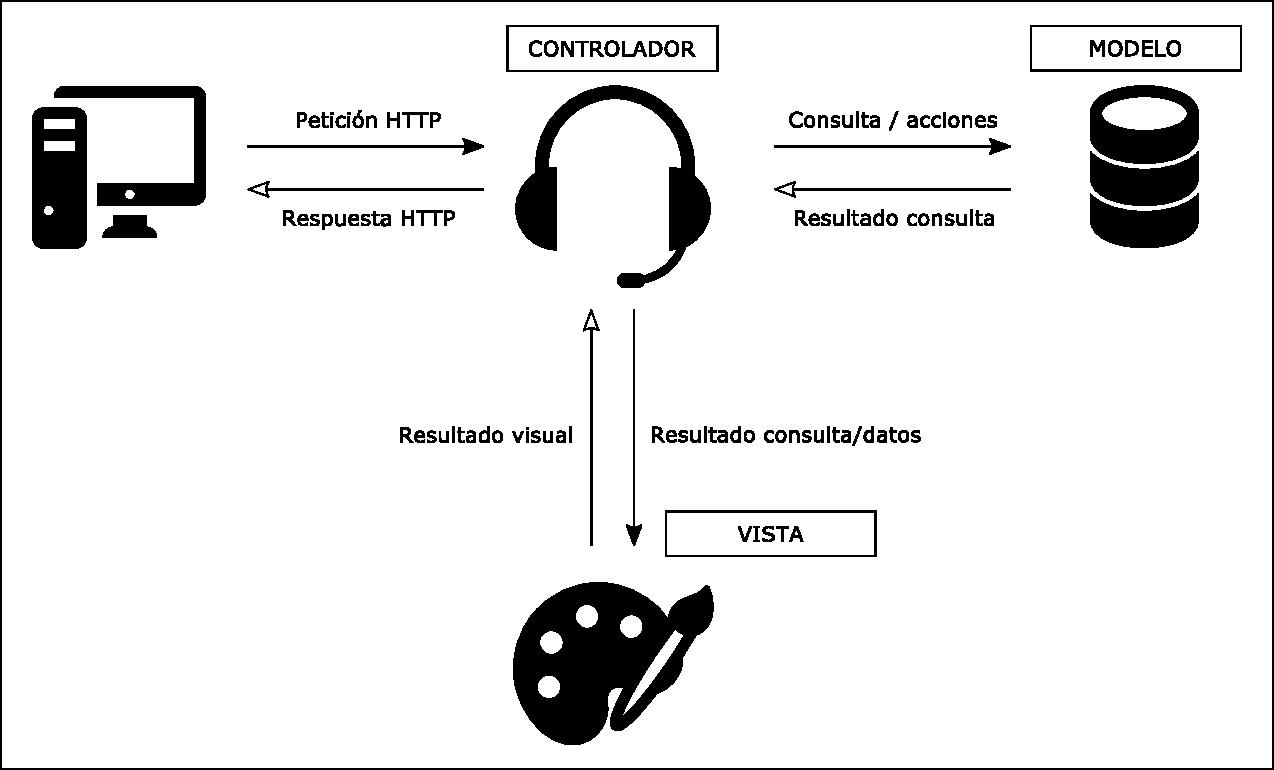
\includegraphics[width=16cm, height=10cm]{figuras/MVC}
		        \caption{Diagrama de flujo de una petici\'on en MVC.}
		        \label{fig_MVC}
		    \end{figure}

		    Los pasos que sigue la petici\'on son los siguientes:
		    \begin{enumerate}

		    	\item El usuario interact\'ua con la interfaz de usuario de alguna forma (por ejemplo, el usuario pulsa un bot\'on, enlace, etc).

		    	\item El controlador recibe (por parte de los objetos de la interfaz-vista) la notificaci\'on de la acci\'on solicitada por el usuario. El controlador gestiona el evento que llega, frecuentemente a trav\'es de un gestor de eventos (handler) o callback. 

		    	\item El controlador accede al modelo, actualiz\'andolo, posiblemente modific\'andolo de forma adecuada a la acci\'on solicitada por el usuario (por ejemplo, el controlador actualiza el carro de la compra del usuario). Los controladores complejos est\'an a menudo estructurados usando un patr\'on de comando que encapsula las acciones y simplifica su extensi\'on. 

		    	\item El controlador delega a los objetos de la vista la tarea de desplegar la interfaz de usuario. La vista obtiene sus datos del modelo para generar la interfaz apropiada para el usuario donde se refleja los cambios en el modelo (por ejemplo, produce un listado del contenido del carro de la compra). El modelo no debe tener conocimiento directo sobre la vista. Sin embargo, se podr\'ia utilizar el patr\'on Observador para proveer cierta indirecci\'on entre el modelo y la vista, permitiendo al modelo notificar a los interesados de cualquier cambio. Un objeto vista puede registrarse con el modelo y esperar a los cambios, pero aun as\'i el modelo en s\'i mismo sigue sin saber nada de la vista. El controlador no pasa objetos de dominio (el modelo) a la vista aunque puede dar la orden a la vista para que se actualice. Nota: En algunas implementaciones la vista no tiene acceso directo al modelo, dejando que el controlador envíe los datos del modelo a la vista.

		    	\item La interfaz de usuario espera nuevas interacciones del usuario, comenzando el ciclo nuevamente.
		    \end{enumerate}


\section{Base de Datos}

	En los \'ultimos tiempos, se ha empezado a considerar la informaci\'on como un recurso estrat\'egico de una organizaci\'on; pues facilita su supervivencia y le permite, adem\'as, ser competitiva en el mercado. Dicha informaci\'on le permite tener una visi\'on de los posibles cambios, y con esto mejorar la toma de decisiones.\\

	Una base de datos se define como una colecci\'on de datos almacenados de una manera permanente, que pueden ser compartidos y usados con distintos prop\'ositos por m\'ultiples usuarios.\\

	La informaci\'on se debe considerar como otro recurso corporativo de la misma manera que se considera el recurso humano o los recursos f\'isicos. Por lo tanto, la administraci\'on de la informaci\'on debe implicar:

	\begin{itemize}
		\item Planear su adquisici\'on por anticipado.
		\item Protegerla contra la destrucci\'on o mal uso.
		\item Asegurar su calidad.
		\item Retirarla de la organizaci\'on cuando ya no se le requiera.
	\end{itemize}


	Debido que la cantidad de informaci\'on que una organizaci\'on necesita para subsistir es cada vez mayor, deben existir m\'etodos eficientes tanto para el almacenamiento r\'apido como para la consulta \'agil. La tecnolog\'ia m\'as utilizada para manejar estas grandes cantidades de informaci\'on son las Bases de Datos.\\

	La tecnolog\'ia de bases de datos proporciona los medios para que se cumplan los objetivos de lograr m\'aximos beneficios en la administraci\'on de informaci\'on debido a las siguientes razones:

	\begin{itemize}
		\item Se logra que el desarrollo de aplicaciones sea m\'as r\'apido debido a que los programadores reutilizan datos u procedimientos almacenados en la base de datos.
		\item Hay una mayor participaci\'on del usuario final en la creaci\'on de las aplicaciones, haciendo software m\'as tangible y de mayor valor inmediato.
		\item El acceso a los datos es flexible y r\'apido.
	\end{itemize}


	Gracias a esto las organizaciones tienen m\'as y mejor informaci\'on para la toma de decisiones, adem\'as de incrementar su productividad.\\

	A continuaci\'on se presentan las ventajas y desventajas de un sistema de base de datos:
	\begin{enumerate}
		\item Ventajas
			\begin{enumerate}
				\item \textbf{Econom\'ia de escala:} esencialmente, la concentraci\'on de aplicaciones en una sola localidad puede reducir costos.
				\item \textbf{Mayor informaci\'on:} existe una mayor facilidad para el an\'alisis y la toma de desiciones.
				\item \textbf{Datos y programas compartidos:} la reutilizaci\'on de los mismos datos y programas, permiten minimizar o controlar la redundancia.
				\item \textbf{Declaraci\'on de est\'andares:} Debido a que la informaci\'on se vuelve muy grande, es necesario declarar est\'andares para el acceso y manejo de los datos.
				\item \textbf{Consistencia de datos:} Esta dada por el control o eliminaci\'on de la redundancia.
				\item \textbf{Integridad:} El sistema de base de datos debe velar por el grado de validez y de correcci\'on de los datos. Debe permitir definir reglas que deben cumplir los datos en la base de datos.
				\item \textbf{Seguridad:} Se pueden especificar niveles de acceso mediante perfiles de usuario.
			\end{enumerate}
		\item Desventajas
			\begin{itemize}
				\item \textbf{Tama\~no:} Un sistema de base de datos es un gran conjunto de programas que a lo largo de su uso su tama\~no incrementa considerablemente.
				\item \textbf{Mayor susceptibilidad a fallas:} Debido a la cantidad de informaci\'on es m\'as probable que se generen fallas.
				\item \textbf{Recuperaci\'on a las fallas:} La recuperaci\'on de un DBMS interactivo y multiusuario puede ser muy compleja.
			\end{itemize}
	\end{enumerate}

	Los sitemas de base de datos utilizan un lenguaje el cual le permite realizar modificaciones sobre ella. Este lenguajes es el llamado SQL.

	\subsection{Lenguaje SQL}

	El lenguaje SQL es un conjunto de onstrucciones que permite crear, consultar y modificar una base de datos. Para realizar estas acciones, SQL se divide en tres grupos de lenguajes de base de datos:
	\begin{itemize}
		\item \textbf{DML (Data Manipulation Language):} Permite consultar y modificar datos.
		\item \textbf{DDL (Data Definition Language):} Permite definir la base de datos.
		\item \textbf{DAL (Data Acces Language):} Permite administrar el acceso a la base de datos.
	\end{itemize}

	Todos los sistemas gestores de base de datos cuentan con estos tres grupos para poder realizar las acciones sobre las bases de datos. Dentro de los sitemas gestores de base de datos mas comunes se encuentran los siguientes:

	\begin{itemize}
		\item SQL Server.
		\item MySQL.
		\item Postgress SQL.
		\item Oracle.
	\end{itemize}

	El lenguaje elegido para realizar el SII es SQL Server, esto debido a la integraci\'on que tiene con el ambiente de desarrollo y los lenguajes seleccionados.

	\subsection{Microsoft SQL Server}

	Microsoft SQL server es un sistema de gesti\'on de bases de datos relacional producido por Microsoft. Su principal lenguaje de consulta es Transact-SQL, una aplicaci\'on de las normas ANSI/ISO estándar Structured Query Language (SQL) utilizando por ambas Microsoft y Sybase.
	
	Las caracter\'isticas de Microsoft SQL Server son las siguientes:
	\begin{itemize}
		\item Soporte de transacciones.
		\item Escalabilidad, estabilidad y seguridad.
		\item Soporta procedimientos almacenados.
		\item Incluye tambi\'en un potente entorno gr\'afico de administraci\'on, que permite el uso de comandos DDL y DML gr\'aficamente.
		\item Permite trabajar en modo cliente-servidor, donde la informaci\'on y datos se alojan en el servidor y las terminales o clientes de la red s\'olo acceden a la informaci\'on.
		\item Adem\'as permite administrar informaci\'on de otros servidores de datos.
	\end{itemize}

	Este sistema incluye una versi\'on reducida, llamada MSDE con el mismo motor de base de datos pero orientado a proyectos m\'as peque\~nos, que en su versi\'on 2005 pasa a ser el SQL Express Edition, que se distribuye en forma gratuita. \\

	Microsoft SQL Server constituye la alternativa de Microsoft a otros potentes sistemas gestores de bases de datos como son Oracle, Sybase ASE, PostgreSQL o MySQL.

		\subsubsection{Requisitos de hardware}

			\begin{table}[H]
			\centering
			\caption{Requisitos de Hardware de Microsoft SQL Server}
			\label{RequisitosSQL}
				\begin{tabular}{ll}
					\hline
						COMPONENTE               & REQUISITO                                                                                                                                                                                                                                                                                                                       \\ \hline
						Memor\'ia                  & \begin{tabular}[c]{@{}l@{}}Minimo:\\ \\ Ediciones Express: 512 MB\\ \\ Todas las dem\'as ediciones: 1 GB\\ \\ Recomendaciones:\\ \\ Ediciones Express: 1 GB\\ \\ Todas las dem\'as ediciones: Al menos 4 GB y debe aumentar a medida que el tama\~no \\ de la base de datos aumente para asegurar un rendimiento \'optimo.\end{tabular} \\ \hline
						Velocidad del procesador & \begin{tabular}[c]{@{}l@{}}Minimo\\ \\ - Procesador x86: 1 GHz.\\ - Procesador x64: 1.4 Ghz.\\ \\ Recomendado: 2 GHz o m\'as.\end{tabular}                                                                                                                                                                                        \\ \hline
						Tipo de procesador       & \begin{tabular}[c]{@{}l@{}}- Procesador x64: AMD Opteron, AMD Athlon 64, Intel Xeon compatible \\ con Intel EM64T Intel Pentium IV.  \\ - Procesador x86: compatible con Pentium III o superior.\end{tabular}                                                                                                                   \\ \hline
				\end{tabular}
			\end{table}

		\subsubsection{Rendimiento}

			Respecto al rendimiento de Microsoft SQL Server, este se desempe\~na dentro de cualquier arquitectura .NET o J2EE.\\

			Del mismo modo este se beneficia de RAID (Redundant Array of Independent Disks) el cual es un sistema de almacenamiento de datos entre los que se distribuye o replican los datos, es decir, este se desempe\~na mejor si se ejecuta en un servidor dedicado espec\'ificamente a \'el.\\

			Microsoft SQL Server como cualquier otro sistema manejador de bases de datos depende de la estructura de las instrucciones que recibe para determinar su rendimiento, esto debido a que existen distintas maneras de consultar o modificar la informaci\'on, es por ello que es importante seguir la documentaci\'on del producto para realizar las instrucciones m\'as r\'apidas posibles.

		\subsubsection{Administraci\'on y mantenimiento}

			Microsoft SQL Server ofrece un grupo de acciones que permiten administrar los recursos dentro del mismo, las cuales se enlistan a continuaci\'on:

			\begin{itemize}
				\item Se provee de un sistema de copias de seguridad en la cual se vuelcan los datos y estructura en un archivo con extensi\'on ".bak".

				\item Soporta tres tipos de replicaci\'n:
					\begin{itemize}
						\item \textbf{Instantanea:} En la replicaci\'on de instant\'aneas los datos se copian tal y como aparecen exactamente en un momento determinado.

						\item \textbf{Transaccional:} En este caso se propaga una instant\'anea inicial de datos a los suscriptores, y despu\'es, cuando se efect\'uan las modificaciones en el publicador, las transacciones individuales se propagan a los suscriptores. Microsoft SQL Server almacena las transacciones que afectan a los objetos replicados y propaga esos cambios a los suscriptores de forma continua o a intervalos programados. Al finalizar la propagaci\'on de los cambios, todos los suscriptores tendr\'an los mismos valores que el publicador.

						\item \textbf{Mixta:} Permite que varios sitios funcionen en l\'inea o desconectados de manera aut\'onoma, y mezclar m\'as adelante las modificaciones de datos realizadas en un resultado \'unico y uniforme. La instant\'anea inicial se aplica a los suscriptores; a continuaci\'on SQL Server 2000 hace un seguimiento de los cambios realizados en los datos publicados en el publicador y en los suscriptores.
					\end{itemize}
			\end{itemize}

		\subsubsection{Estabilidad}

			Microsoft SQL Server tiene una gran resistencia a la corrupci\'on de datos  ya que los datos van a trav\'es de distintos puestos de control y previene contratiempos en caso de que el sistema colapse sin previo aviso. Se puede considerar como un contratiempo a un fallo inesperado del equipo hu\'esped de Microsoft SQL Server o un apagado inesperado del mismo.

		\subsubsection{Desarrollo de aplicaciones}

			\begin{itemize}
				\item Se cuenta con m\'ultiples APIs para acceder a \'el.
				\item Se apoya en ODBC y JDBC para conectividad en red, as\'i como los m\'etodos de acceso de base de datos nativos.
				\item Soporta conexiones desde distintos lenguajes como C/C++, Java, Perl, Python, PHP, C\# y Visual Basic.
				\item Soporta m\'etodos de cifrado SSL.
			\end{itemize}

		\subsubsection{Licencias}

			El licenciamiento de Microsoft SQL Server esta disponible de las siguientes dos maneras:
			\begin{itemize}
				\item \textbf{Por Procesador:} Requiere una licencia \'unica para cada CPU en el equipo que ejecuta e incluye el acceso limitado de clientes.
				\item \textbf{Servidor/por asiento:} Se requiere una licencia para el servidor y las licencias para cada cliente.
			\end{itemize}

	Ya terminados los putos de la parte técnica del proyecto, hablaremos de la parte de la metodología utilizada para realizar el mismo.

\section{Metodolog\'ia de desarrollo}

	Se le llama metodolog\'ia a el conjunto de t\'ecnicas y herramientas que dan una documentaci\'on formal al proyecto referente a los procesos, las pol\'iticas y procedimientos que ayudan a los desarrolladores para la realizaron de un producto (software) .\\

	El objetivo principal de una metodolog\'ia es tener mayor eficacia al cumplir con los requisitos que se plantearon desde un principio en el proyecto, adem\'as  de prevenir las p\'erdidas de tiempo en la realizaci\'on del mismo, siendo un gu\'ia que llevar\'a de manera ordenada el equipo de trabajo en el desarrollo de software con respecto a las actividades y a que el software tiene un ciclo de vida, es decir, tiene un tiempo l\'imite para su cumplimiento.\\

	De forma general el ciclo de vida del software est\'a definido de los siguientes puntos:
	\begin{itemize}
		\item \textbf{Definici\'on de objetivos:} se definen todas las ideas concretas del proyecto permitiendo tener una visi\'on general del mismo, adem\'as de establecer un panorama amplio para la definici\'on de alcances.
		\item \textbf{An\'alisis de requisitos y su viabilidad:} Se recopilan los requisitos del cliente y examina cualquier restricci\'on que se pueda aplicar, es aqu\'i donde se comienzan a visualizar los alcances del proyecto.
		\item \textbf{Dise\~no general:} Son los requisitos generales de la arquitectura del proyecto.
		\item \textbf{Dise\~no en detalle:} Es la definici\'on precisa de cada bloque de la aplicaci\'on, esto hace referencia al detalle del funcionamiento y acciones a realizar por el sistema.
		\item \textbf{Programaci\'on:} Es la implementaci\'on de un lenguaje de programaci\'on para crear los modulos o funciones definidas en el proyecto.
		\item \textbf{Prueba de unidad:} Es la prueba individual de cada bloque para verificar que cumplen con las especificaciones de dise\~no y funcionalidad del proyecto.
		\item \textbf{Prueba beta:} Esta prueba se encarga de garantizar que el software cumple con las especificaciones originales y cumpla con todos los objetivos establecidos.
		\item \textbf{Documentaci\'on:} Es la gu\'ia que servir\'a a los usuarios que utilizaran el software a aclarar sus dudas respecto al funcionamiento del mismo en caso de usuarios finales, adem\'as de la creaci\'on de un manual t\'ecnico que servir\'a como gu\'ia para los encargados del soporte.
		\item \textbf{Implementaci\'on:} Es la puesta en marcha del proyecto para su uso, para llegar a esta parte es necesario que los puntos anteriores se evaluaran de manera satisfactoria y con esto validar que el software esta listo para ponerse en un ambiente de producci\'on.
		\item \textbf{Mantenimiento:} Es la correcci\'on de los posibles errores resultantes del uso cotidiano de los usuarios finales, estos se pueden presentar de dos maneras, errores de datos y errores de sistema. 
		\begin{itemize}
			\item Los errores de datos hacen referencia a una mala captura de informaci\'on por parte del sistema o el usuario final, truncando con esto alguno de los procesos posteriores debido a informaci\'on incorrecta o falta de la misma.
			\item Los errores de sistema son aquellos en los que la falla es ocasionada por un fallo directamente en la programaci\'on del sistema.
		\end{itemize}

	\end{itemize}

	Los modelos para el desarrollo de software est\'an clasificados en tres grupos, de los cuales cada uno de ellos representa el proceso de desarrollo de software de una manera particular, y a pesar de estar definidos claramente, no representan necesariamente la realidad de c\'omo  se debe desarrollar el software, si no que establece un enfoque com\'un. Un modelo puede ser modificado y adaptado de acuerdo a las necesidades de software en desarrollo.\\

	Los tres grupos de modelos de desarrollo son los siguientes:
	\begin{itemize}
		\item Modelo en cascada.
		\item Modelo evolutivo.
		\item Modelo basado en componentes.
	\end{itemize}

	El modelo que se utilizar\'a para el desarrollo de este proyecto es el modelo en cascada, del cual hablaremos a continuaci\'on.

	\subsection{Modelo en cascada}

	Modelo conocido tambi\'en como modelo cl\'asico, modelo tradicional o modelo lineal secuencial.\\

	Es el m\'as b\'asico de todos los modelos y sirve como bloque de construcci\'on para los dem\'as paradigmas de ciclo de vida del desarrollo de sistemas, se puede decir que es un m\'etodo puro que implica un desarrollo r\'igido y lineal. Est\'a basado en el ciclo convencional de una ingenier\'ia y su visi\'on es muy simple: el desarrollo de software se debe realizar siguiendo una secuencia de fases. Cada etapa tiene un conjunto de metas bien definidas y las actividades dentro de cada una contribuyen a la satisfacci\'on de metas de esa.

	Las fases normalmente aplicadas son:
	\begin{itemize}
		\item \textbf{An\'alisis del Sistema:} En esta fase se establecen los requisitos de todos los elementos del sistema y luego se asigna alg\'un subconjunto de estos requisitos al software.
		\item \textbf{An\'alisis de requisitos del software:} El proceso de recopilaci\'on de los requisitos se centra e intensifica especialmente en el software. Es necesario comprender el \'ambito de la informaci\'on del software as\'i como la funci\'on, el rendimiento y las interfaces requeridas.
		\item \textbf{Dise\~no del sistema:} Se enfoca en cuatro atributos distintos del programa: 
			\begin{itemize}
				\item La estructura de los datos.
				\item La arquitectura del software.
				\item El detalle procedimental.
				\item La caracterizaci\'on de la interfaz. 
			\end{itemize}
		\item \textbf{Codificaci\'on:} El dise\~no debe traducirse en una forma legible para la m\'aquina. Si el dise\~no se realiza de una manera detallada, la codificaci\'on puede realizarse mec\'anicamente.
		\item \textbf{Pruebas:} Generado el c\'odigo se inicia la prueba del programa. Que se centra en la l\'ogica interna del software y en las funciones externas, realizando pruebas que aseguren que la entrada definida produce los resultados que realmente se requieren.
		\item \textbf{Implantaci\'on:} Significa programaci\'on. Producto de esta etapa es el c\'odigo en cualquier nivel, incluido el producido por sistemas de generaci\'on autom\'atica.
		\item \textbf{Mantenimiento:} el software  puede sufrir\'a algunos cambios despu\'es de que se entrega al cliente. Los cambios ocurrir\'an debidos a que se haya encontrado errores, a que el software deba adaptarse a cambios del entorno externo (sistema operativo o dispositivos perif\'ericos) o a que el cliente requiera ampliaciones funcionales o del rendimiento.
	\end{itemize}


	Sin embargo debemos saber que los proyectos reales raramente siguen el flujo secuencial que propone el modelo. Siempre hay iteraciones y se crean problemas en la aplicaci\'on del paradigma.\\

	Es dif\'icil para el cliente establecer todos los requisitos expl\'icitamente. El ciclo de vida cl\'asico lo requiere y tiene dificultades en acomodar posibles incertidumbres que pueden existir al comienzo de muchos productos. \\

	Por lo tanto se inicia con la especificaci\'on de requerimientos del cliente, continua con la planificaci\'on, el modelado, la construcci\'on y el despliegue para finalizar en el enfoque del software. El modelo está dirigido por documentos y no proporciona resultados tangibles de software hasta el final del ciclo de vida de algunas herramientas. El dise\~no en cascada es una secuencia definida de los acontecimientos y los resultados finales para proporcionar una estructura para cualquier proyecto que siga el contenido espec\'ifico y detallado. Puede ser apropiado para proyectos de software que son estables especialmente cuando sus requisitos no cambian. Es caracterizado por ordenar de manera rigurosa las etapas del ciclo de vida de software, dado que el comienzo de cada etapa debe esperar a la finalizaci\'on de la inmediata anterior.\\

	La metodolog\'ia en cascada es esencialmente:
	\begin{itemize}
		\item El inicio y el alcance del proyecto.
		\item La planificaci\'on del proyecto (calendario, recursos necesarios, costo).
		\item Definici\'on de las necesidades del negocio y el an\'alisis en detalle de la soluci\'on.
		\item La creaci\'on de la soluci\'on.
		\item Prueba que la soluci\'on funciona.
		\item La entrega de la soluci\'on a su p\'ublico objetivo.
		\item Cierre del proyecto.
	\end{itemize}

	\subsubsection{Ventajas}
	\begin{itemize}
		\item Permite el control de gesti\'on.
		\item Plazos normalmente adecuados para cada etapa de desarrollo.
		\item Este proceso conduce a entregar el proyecto a tiempo.
		\item Es sencilla y facilita la gesti\'on de proyectos.
		\item Permite tener bajo control el proyecto.
		\item Limita la cantidad de interacci\'on entre equipos que se produce durante el desarrollo.
	\end{itemize}


	\subsubsection{Desventajas}
	\begin{itemize}
		\item No conocer si la soluci\'on es correcta hasta estar cerca de su lanzamiento.
		\item Poco tiempo para corregir fallas.
		\item Depuraci\'on complicada.
		\item Los cambios introducidos durante el desarrollo pueden confundir al equipo.
		\item No es frecuente que el cliente o usuario final explicite clara y completamente los requisitos.
		\item Es necesaria la paciencia del cliente.
		\item El cliente podr\'ia detectar un error.
		\item El proceso es lento y pesado.
	\end{itemize}

	\subsubsection{Probable fracaso del modelo de cascada}
	\begin{itemize}
		\item Los clientes quieren ver el producto a medida que se desarrolla.
		\item El cliente no puede validar el producto a medida que lo desarrollamos.
		\item No poder tomas decisiones por la falta de avances o resultados.
		\item Las actividades est\'an estrictamente ligadas causando as\'i impedir que una actividad empiece antes determinar totalmente la anterior, provocando invertir alg\'un tiempo de desarrollo innecesariamente.
	\end{itemize}

